\section{Data description}
\subsection{Dataset overview}
The two source forms contain 1,126 responses. Target cleaning removes 18 rows without a usable CGPA response, giving 1,108 final records. Table~\ref{tab:composition} reports the institutional composition.

\begin{table}[H]\centering
\caption{Dataset composition after target cleaning.}\label{tab:composition}
\begin{tabular}{lrr}\toprule University&Records&Share (\%)\\\midrule
KUET&878&79.2\\BUET&104&9.4\\BRAC University&101&9.1\\CUET&25&2.3\\\midrule Total&1,108&100.0\\\bottomrule
\end{tabular}
\end{table}

\begin{figure}[H]\centering
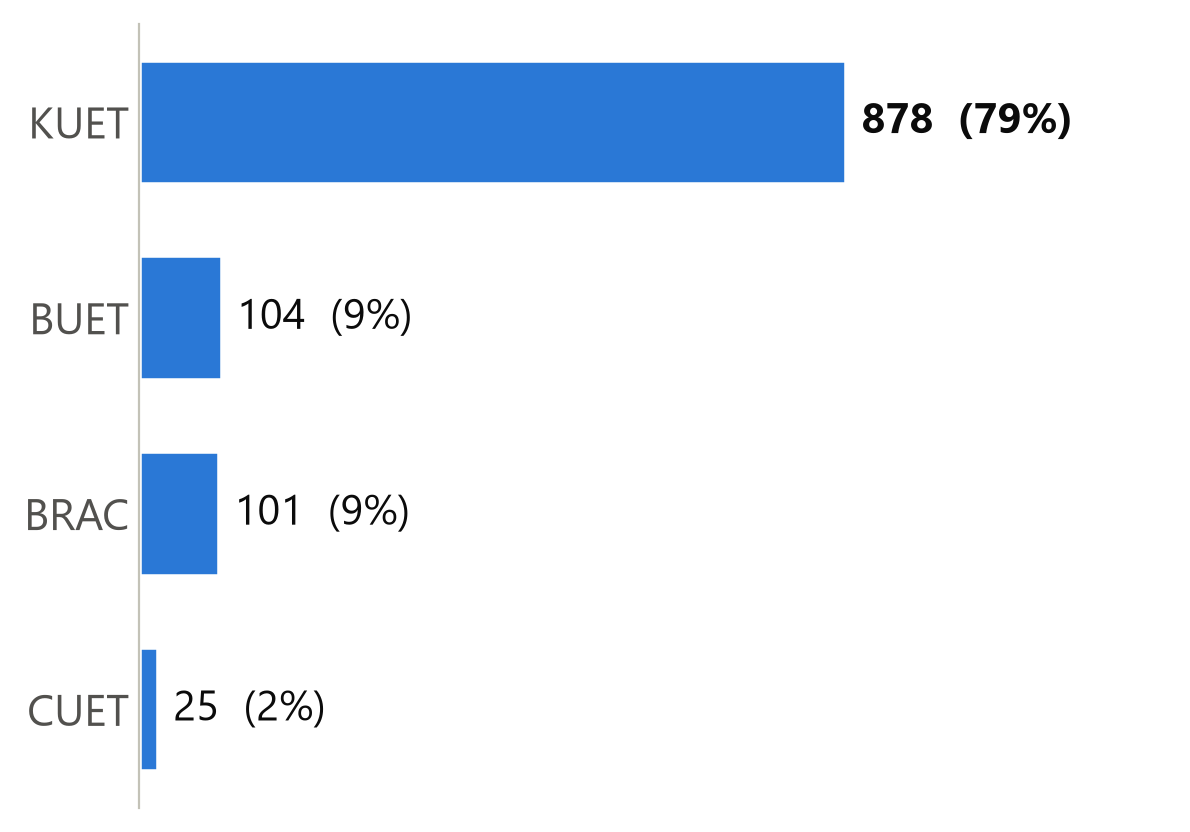
\includegraphics[width=0.84\textwidth]{figures/university_distribution.png}
\caption{University distribution in the cleaned dataset.}
\label{fig:university}
\end{figure}

\subsection{Questionnaire structure}
The common questionnaire covers academic context, study habits, lifestyle, pressure, motivation, support, environment, and grade outcomes. The two forms ask the same core questions but do not always use identical English text or answer formatting. Figure~\ref{fig:form} shows representative form content. No names or roll numbers appear in the modelling table.

\begin{figure}[H]\centering
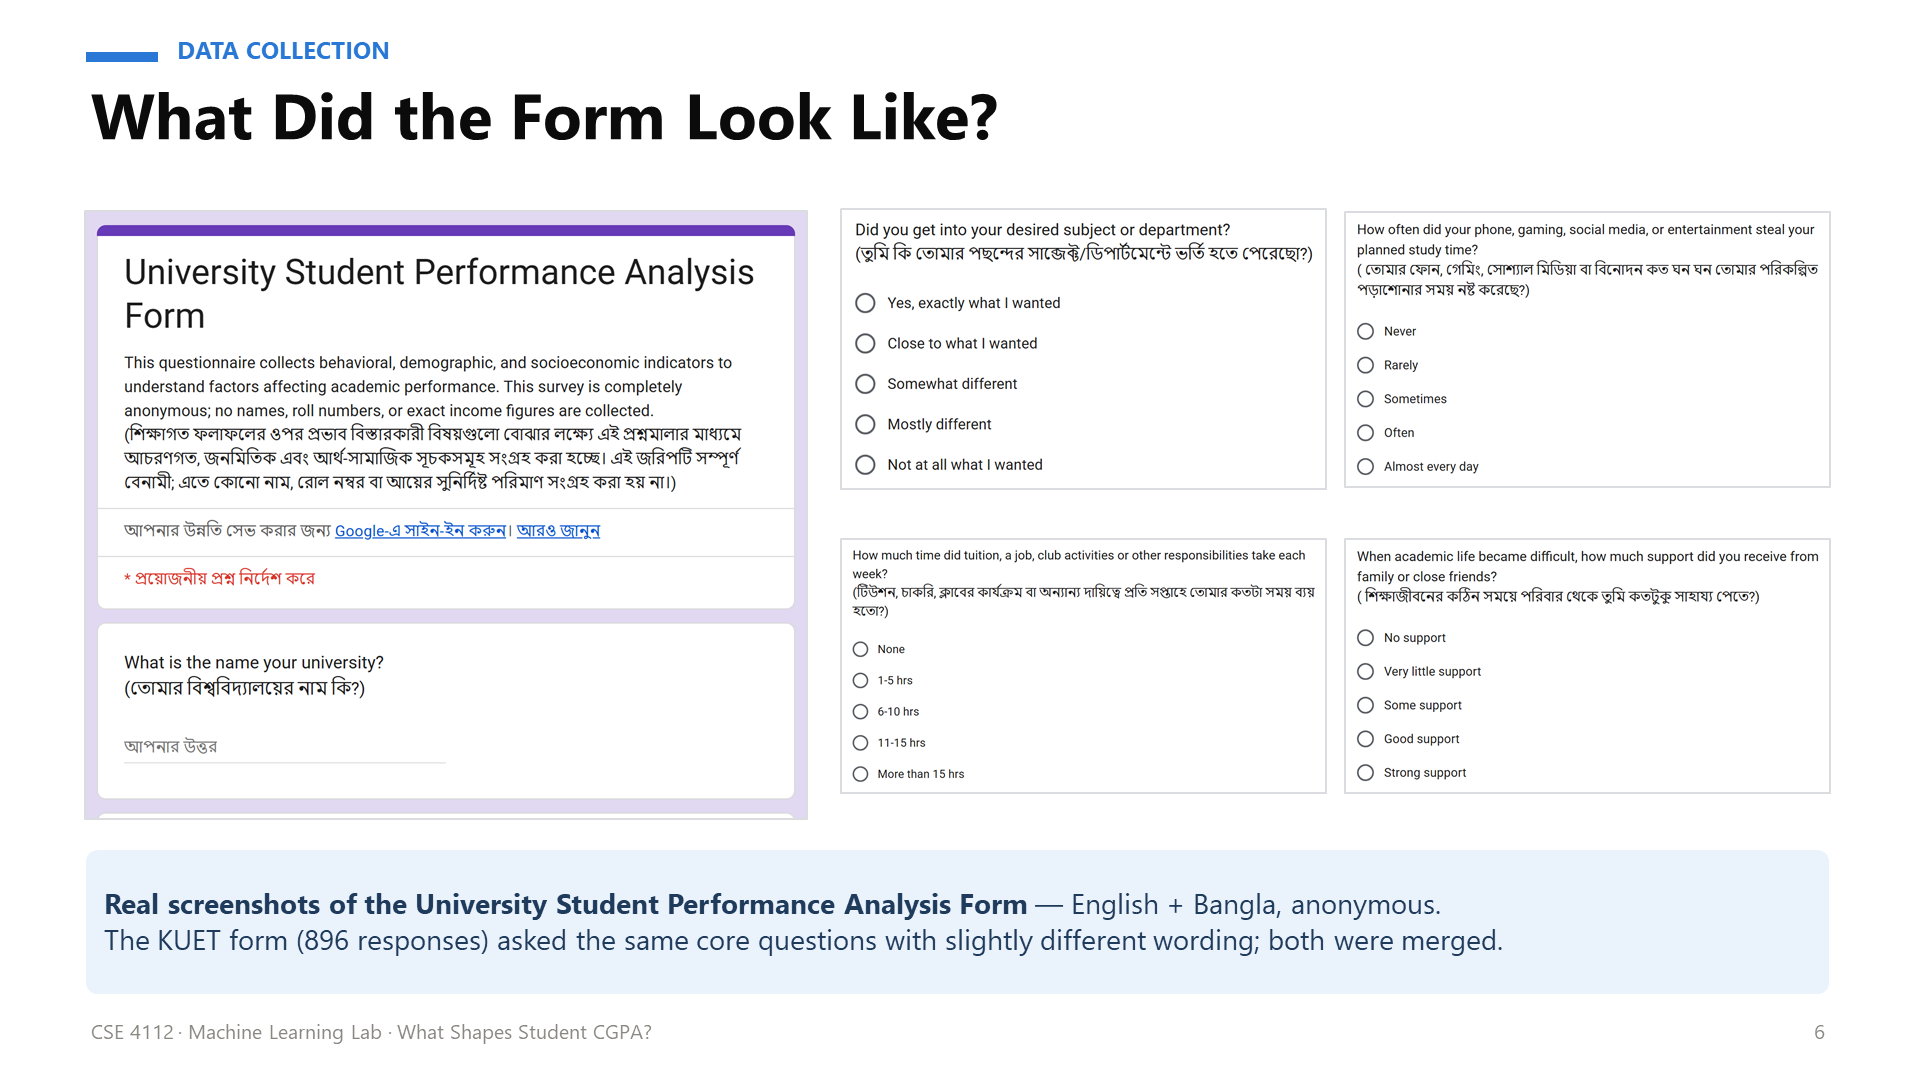
\includegraphics[width=0.95\textwidth]{figures/form_overview.png}
\caption{Representative form questions from the multi-university questionnaire. The KUET form used the same core concepts with some different wording.}
\label{fig:form}
\end{figure}

\begin{table}[H]\centering\small
\caption{Questionnaire variable groups.}\label{tab:variables}
\begin{tabularx}{\textwidth}{p{0.20\textwidth}Yp{0.24\textwidth}}\toprule
Group&Variables&Typical response form\\\midrule
Academic&University, department, semester, recent SGPA, CGPA&Nominal fields and ordered bands\\
Study habits&Attendance, weekly study time, study style, topic clarity&Five ordered categories\\
Lifestyle&Sleep duration, phone or social-media distraction&Five ordered categories\\
Pressure&Stress frequency, outside commitments&Frequency or hour bands\\
Motivation and support&Desired department, admission satisfaction, career expectation, family or friend support&Five ordered categories\\
Environment&Study-friendly living place, routine manageability&Five ordered categories\\\bottomrule
\end{tabularx}
\end{table}

\subsection{Response distributions}
All descriptive counts use the complete 1,108-row cleaned snapshot. For example, 418 students (37.7\%) report attendance of 90\% or more, 302 (27.3\%) report that stress sometimes blocks study, and 310 (28.0\%) report five to six hours of sleep. These figures describe answer frequencies only.

\begin{figure}[H]
\centering
\begin{subfigure}{0.49\textwidth}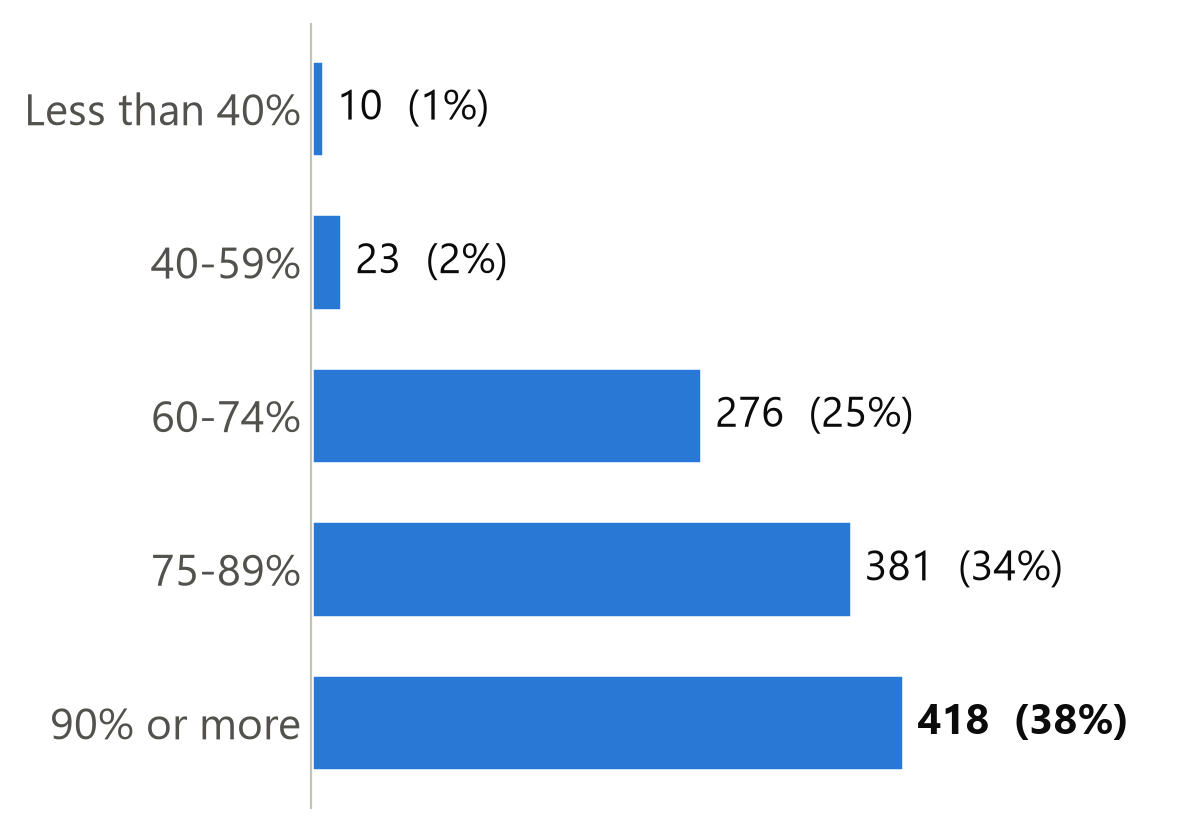
\includegraphics[width=\linewidth]{figures/attendance_distribution.png}\caption{Attendance}\end{subfigure}
\begin{subfigure}{0.49\textwidth}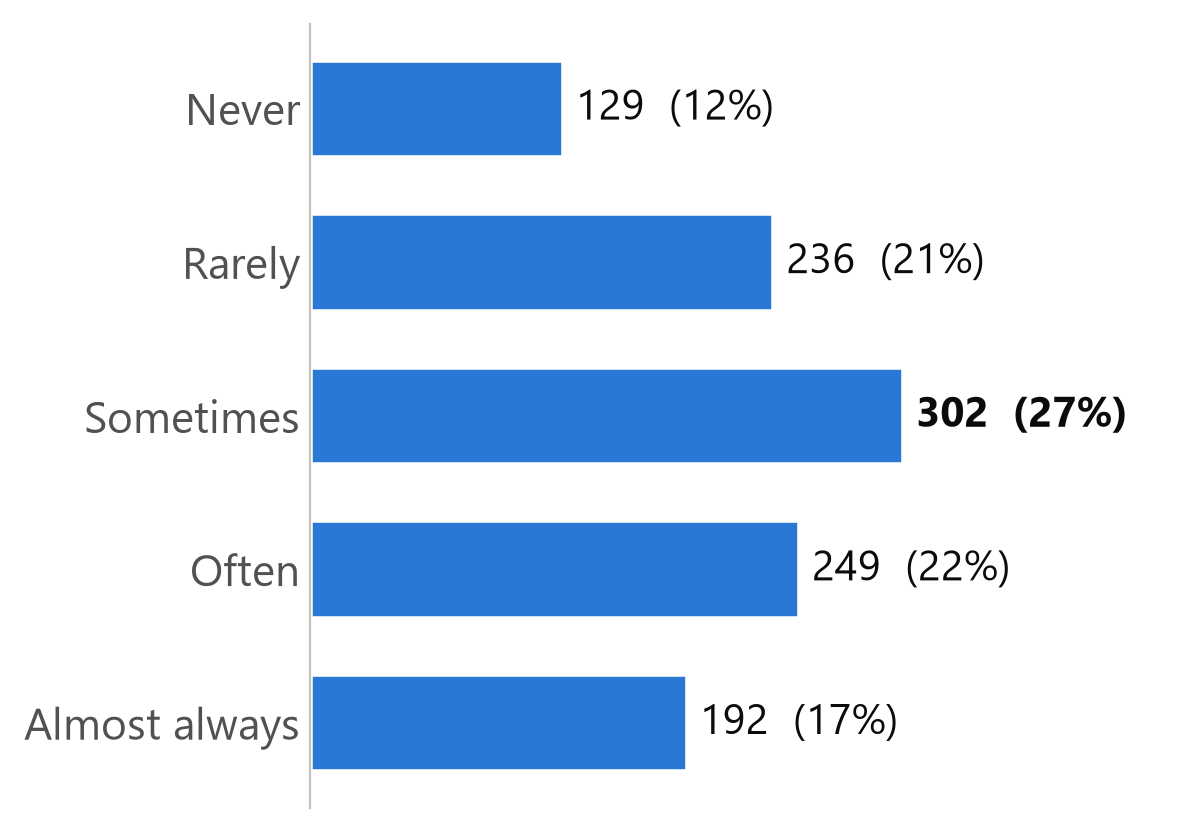
\includegraphics[width=\linewidth]{figures/stress_distribution.png}\caption{Stress frequency}\end{subfigure}
\caption{Examples of cleaned questionnaire response distributions.}
\label{fig:responses-a}
\end{figure}

\begin{figure}[H]\centering
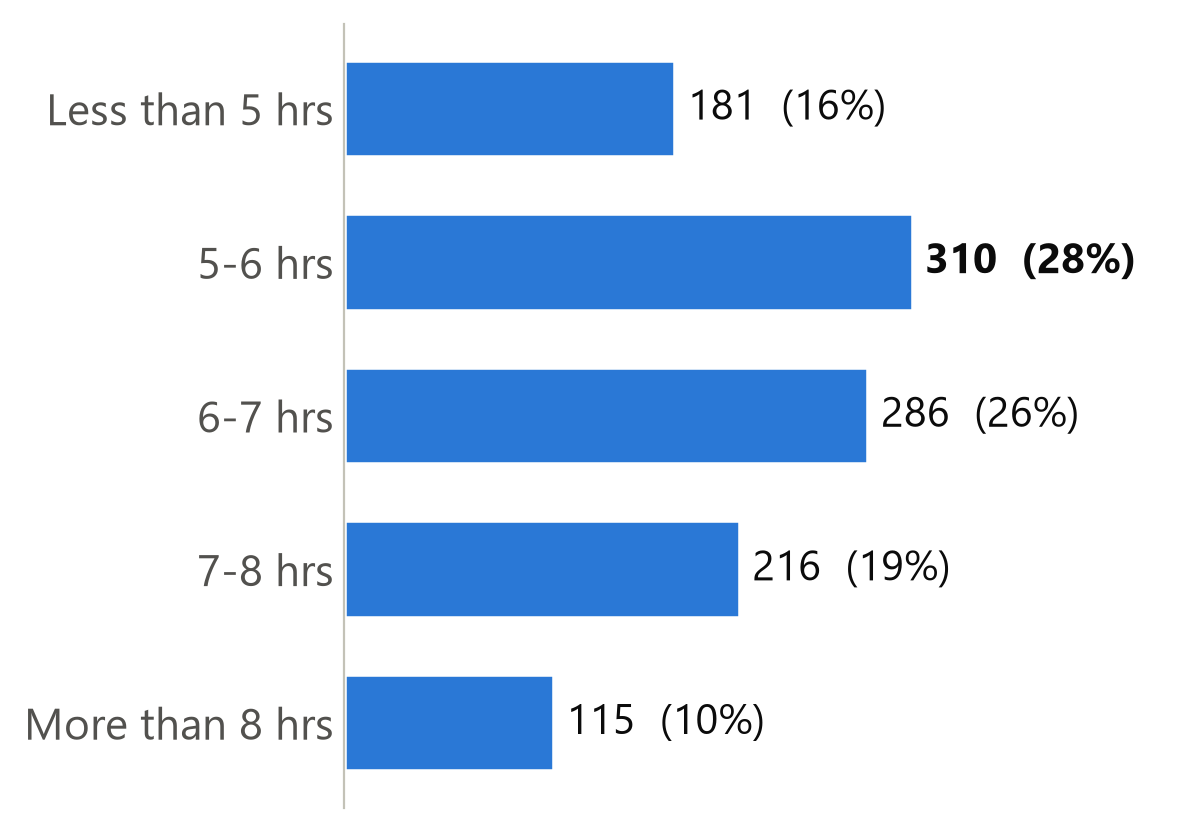
\includegraphics[width=0.72\textwidth]{figures/sleep_distribution.png}
\caption{Reported sleep duration in the cleaned dataset.}
\label{fig:sleep}
\end{figure}

\subsection{Target classes}
Both forms record grade ranges rather than a consistent exact numeric CGPA. The common target is therefore an ordered four-class variable.
\begin{table}[H]\centering
\caption{CGPA target groups.}\label{tab:classes}
\begin{tabular}{llrr}\toprule Code&CGPA range&Count&Share (\%)\\\midrule
C0&Below 3.20&236&21.3\\C1&3.20--3.49&321&29.0\\C2&3.50--3.74&303&27.3\\C3&3.75 and above&248&22.4\\\bottomrule
\end{tabular}
\end{table}
\begin{figure}[H]\centering
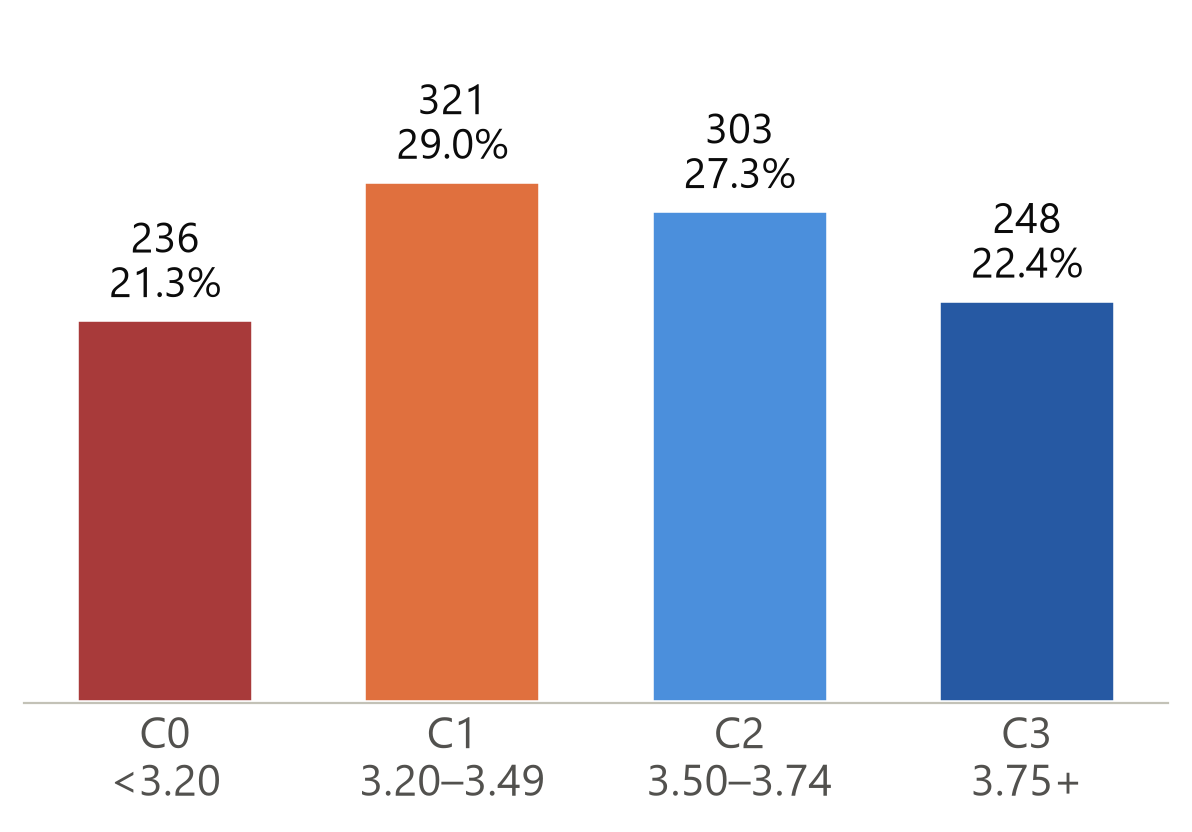
\includegraphics[width=0.72\textwidth]{figures/cgpa_distribution.png}
\caption{Distribution of the four CGPA target groups.}
\label{fig:cgpa-dist}
\end{figure}

\subsection{Reference dataset comparison}
The IUBAT reference dataset contains 894 Computer Science students and 31 columns, including exact numeric CGPA and SGPA, attendance, study hours, social-media hours, co-curricular activity, and socioeconomic variables \cite{prama2024}. The current questionnaire uses grade bands and adds direct questions about stress, sleep, topic clarity, desired department, support, study environment, and routine manageability.
\begin{figure}[H]\centering
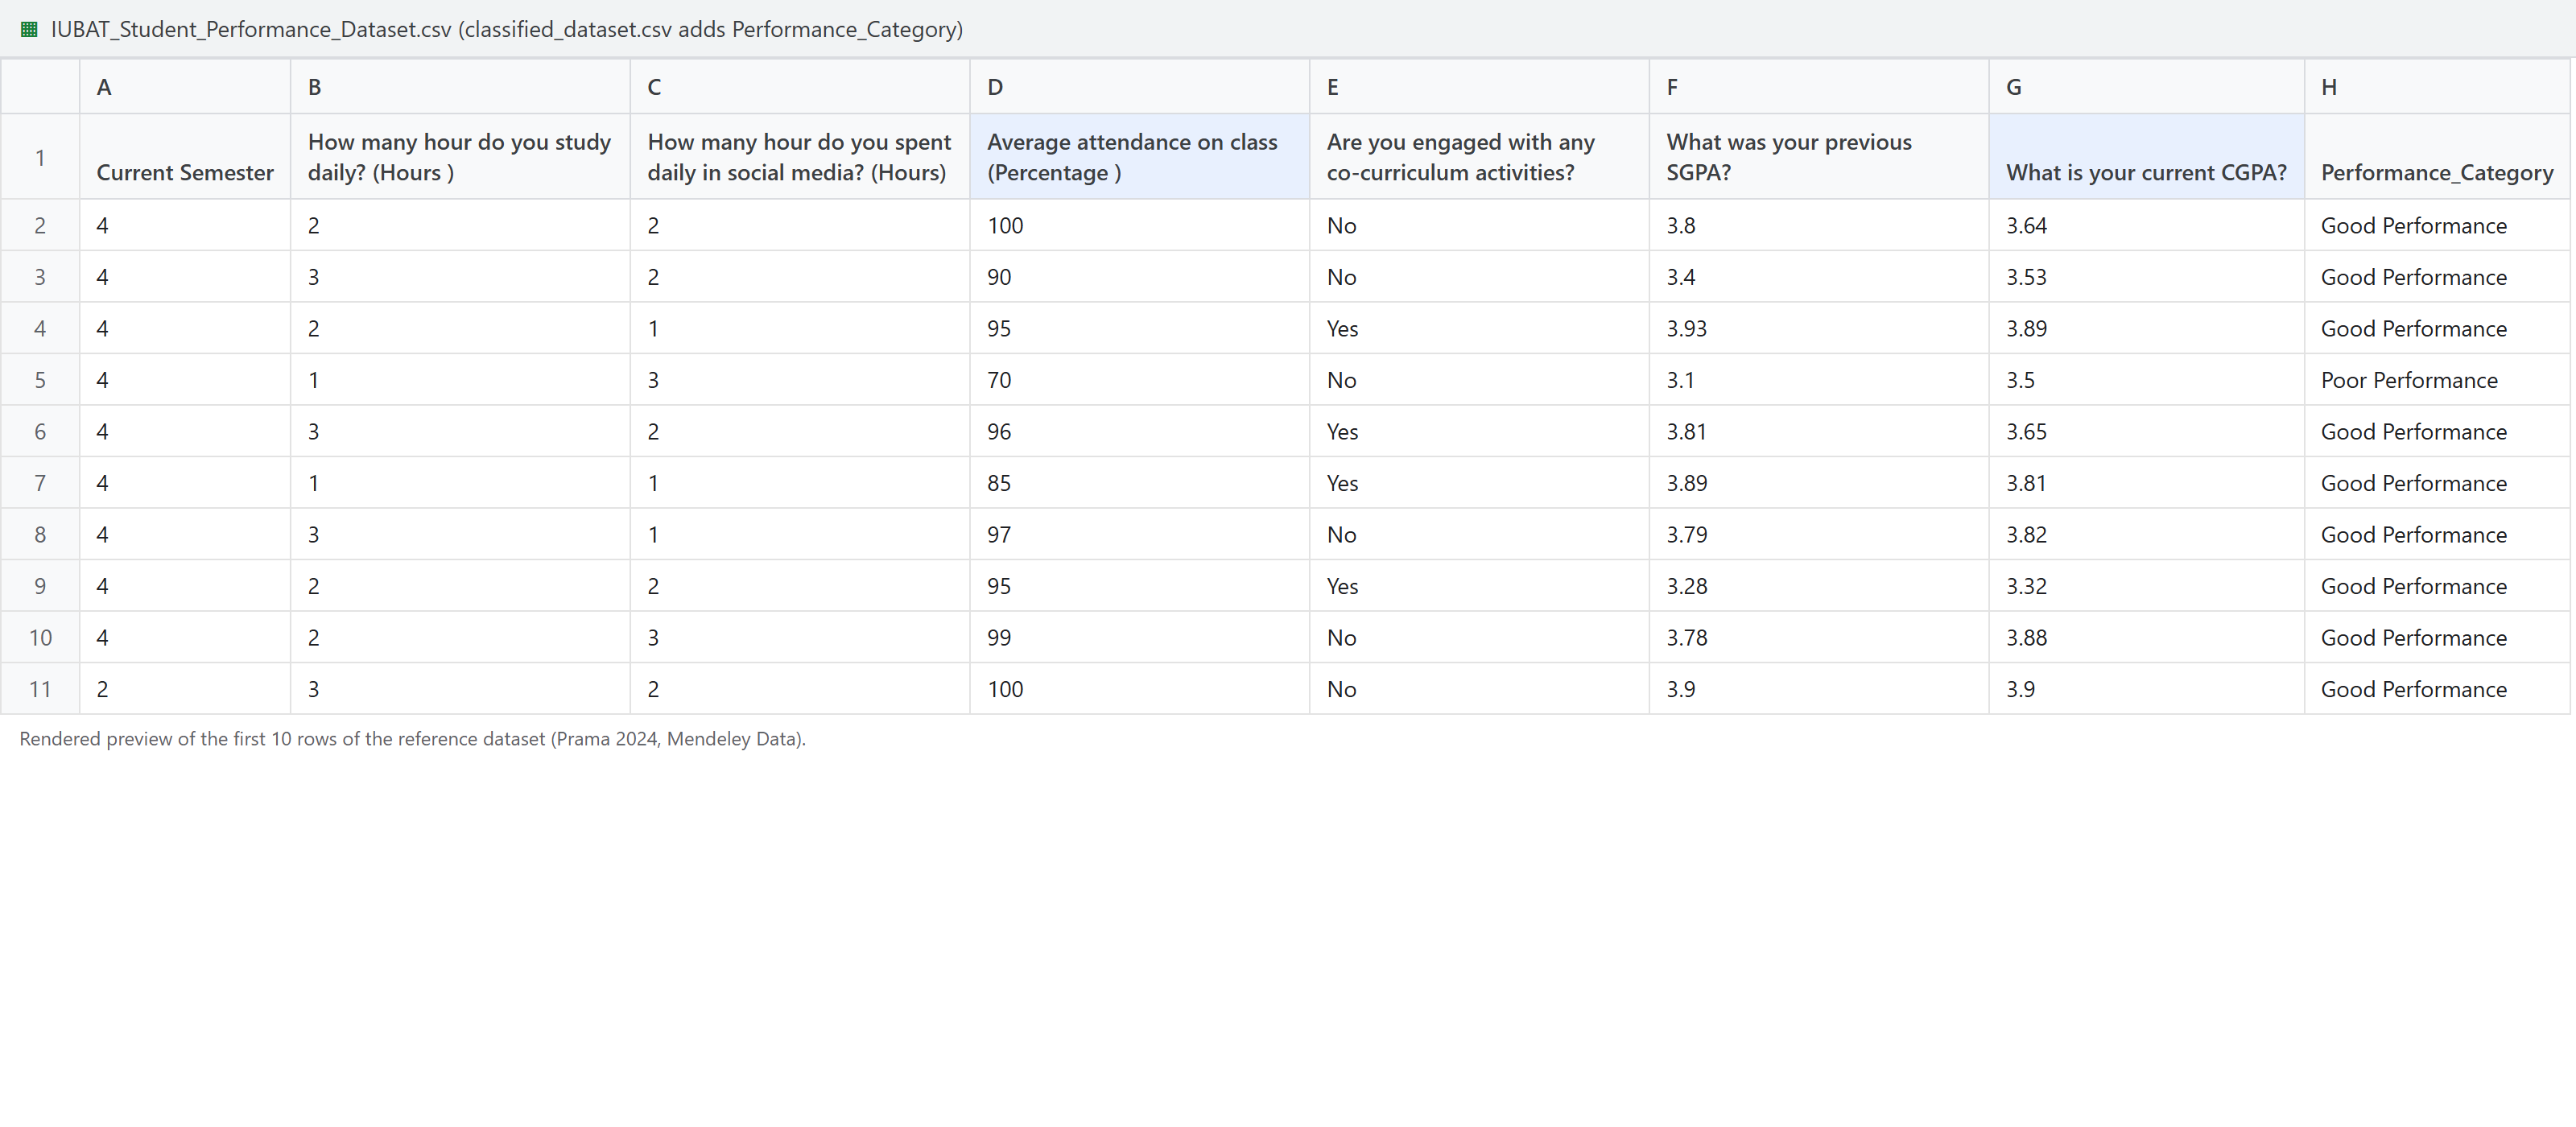
\includegraphics[width=0.95\textwidth]{figures/reference_dataset_preview.png}
\caption{Preview of the IUBAT reference dataset used to compare feature coverage.}
\label{fig:reference-preview}
\end{figure}

\subsection{Files and reproducibility}
The project package contains raw response files, three cleaned merged tables, WEKA-ready CSV and ARFF files, executed notebooks, machine-readable result summaries, figures, a data dictionary, cleaning logs, fixed split indices, and WEKA output logs. Figure~\ref{fig:dataset-preview} illustrates the cleaned row structure.
\begin{figure}[H]\centering
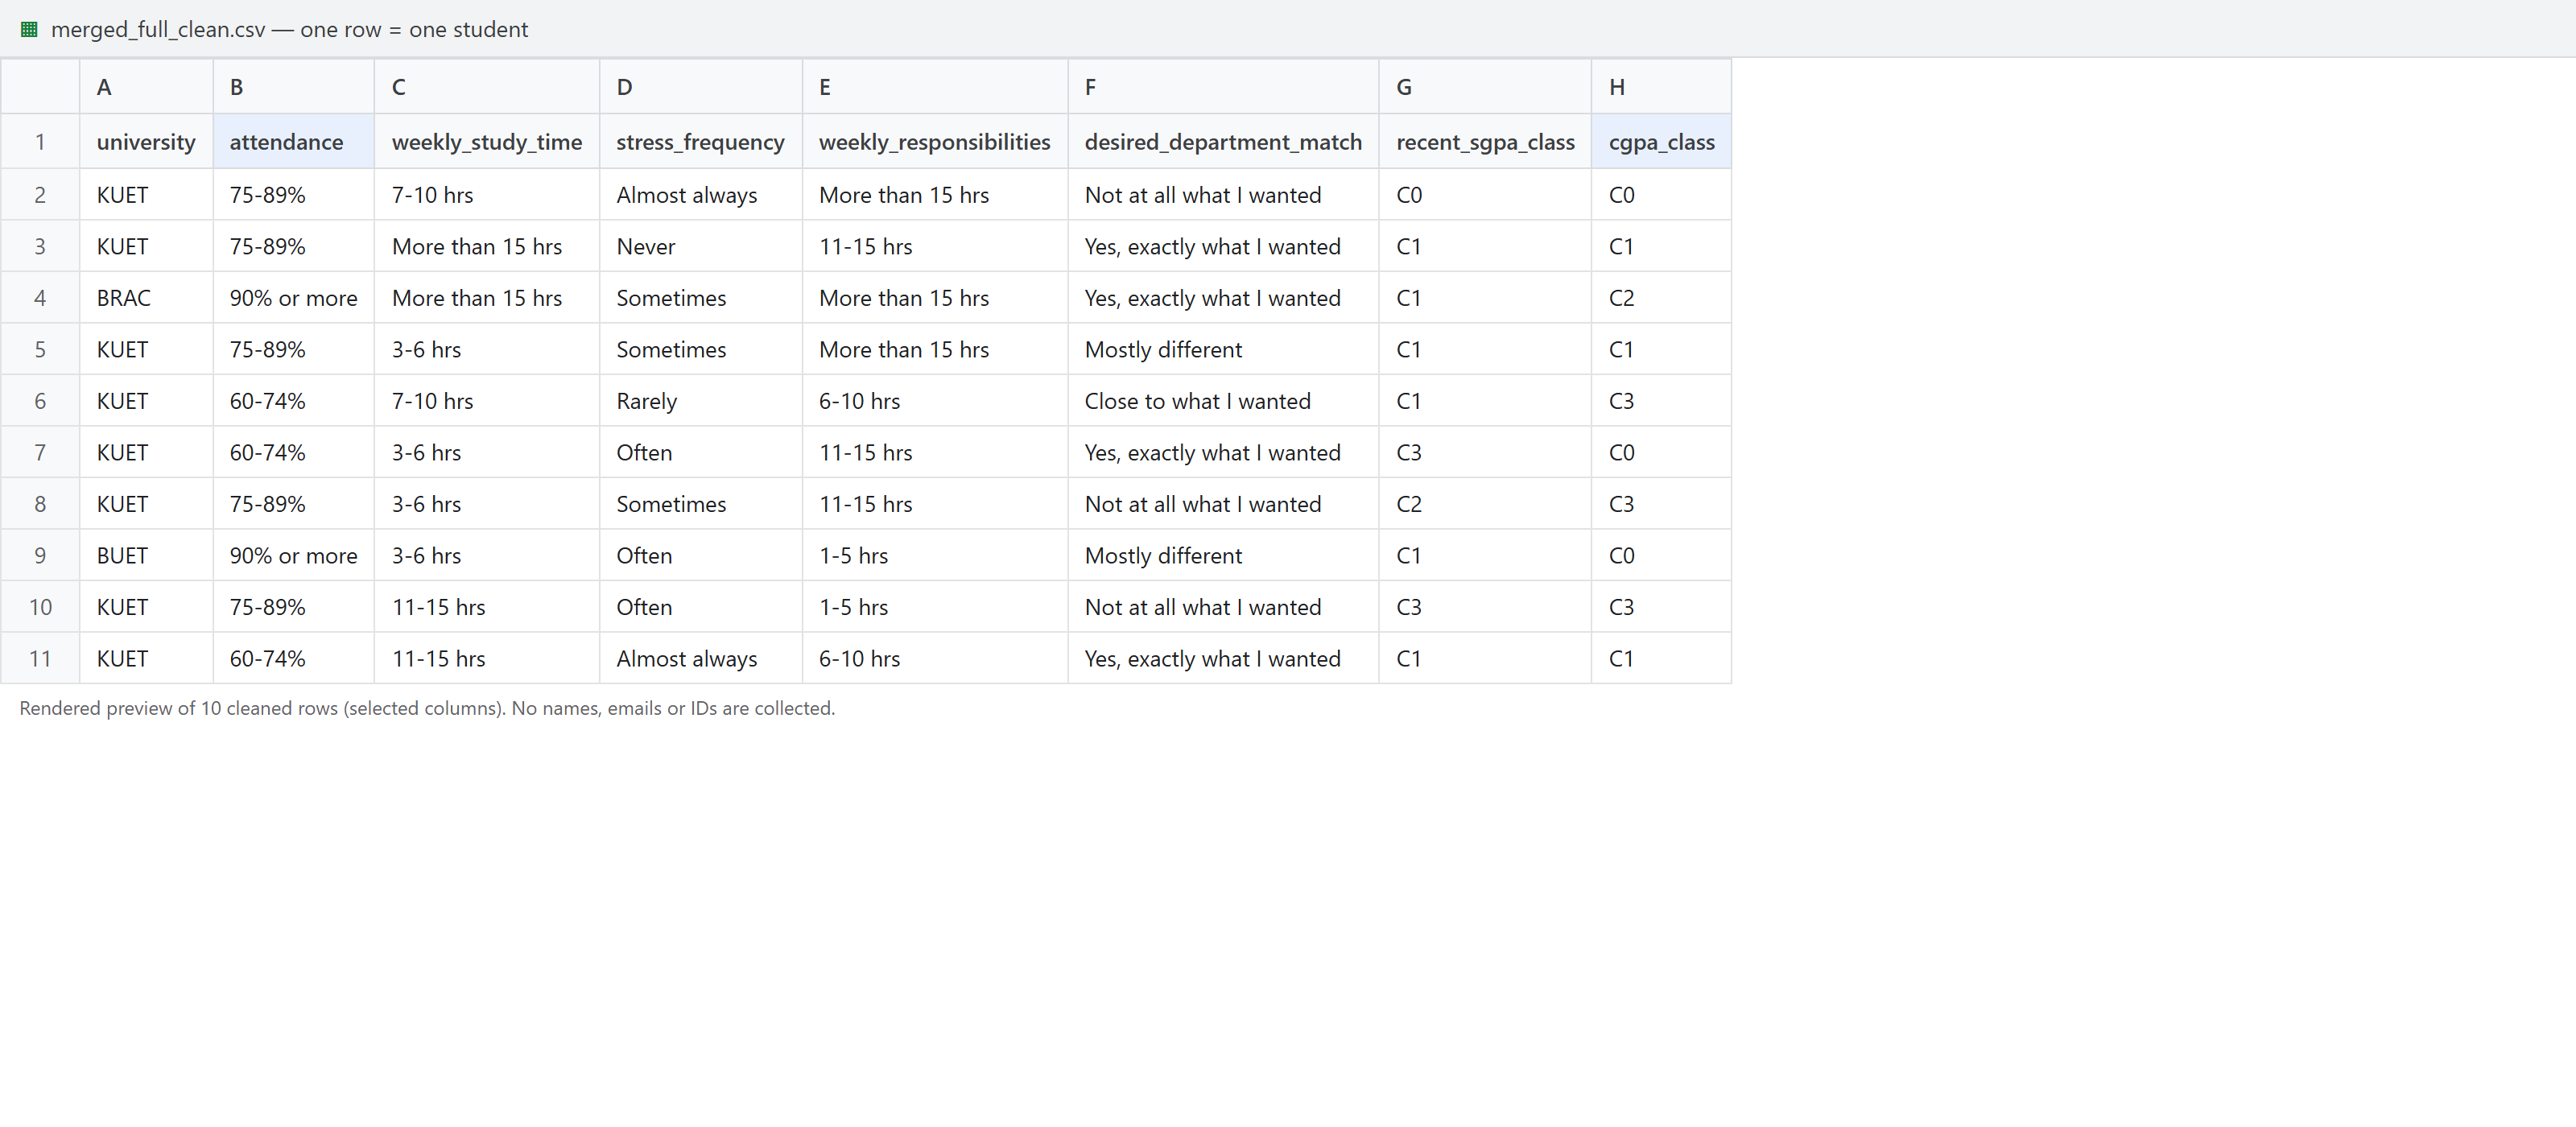
\includegraphics[width=0.95\textwidth]{figures/dataset_preview.png}
\caption{Cleaned dataset preview. One row represents one student response.}
\label{fig:dataset-preview}
\end{figure}

